\documentclass[../main.tex]{subfiles}
\begin{document}
Um den Umfang der Anforderung an die \glspl{CCC} zu verstehen, muss erst ein Verständnis für die Entwicklung der SAP Produkte und damit auch für die Produkte selbst entstehen.

\begin{figure}[ht]
    \centering
    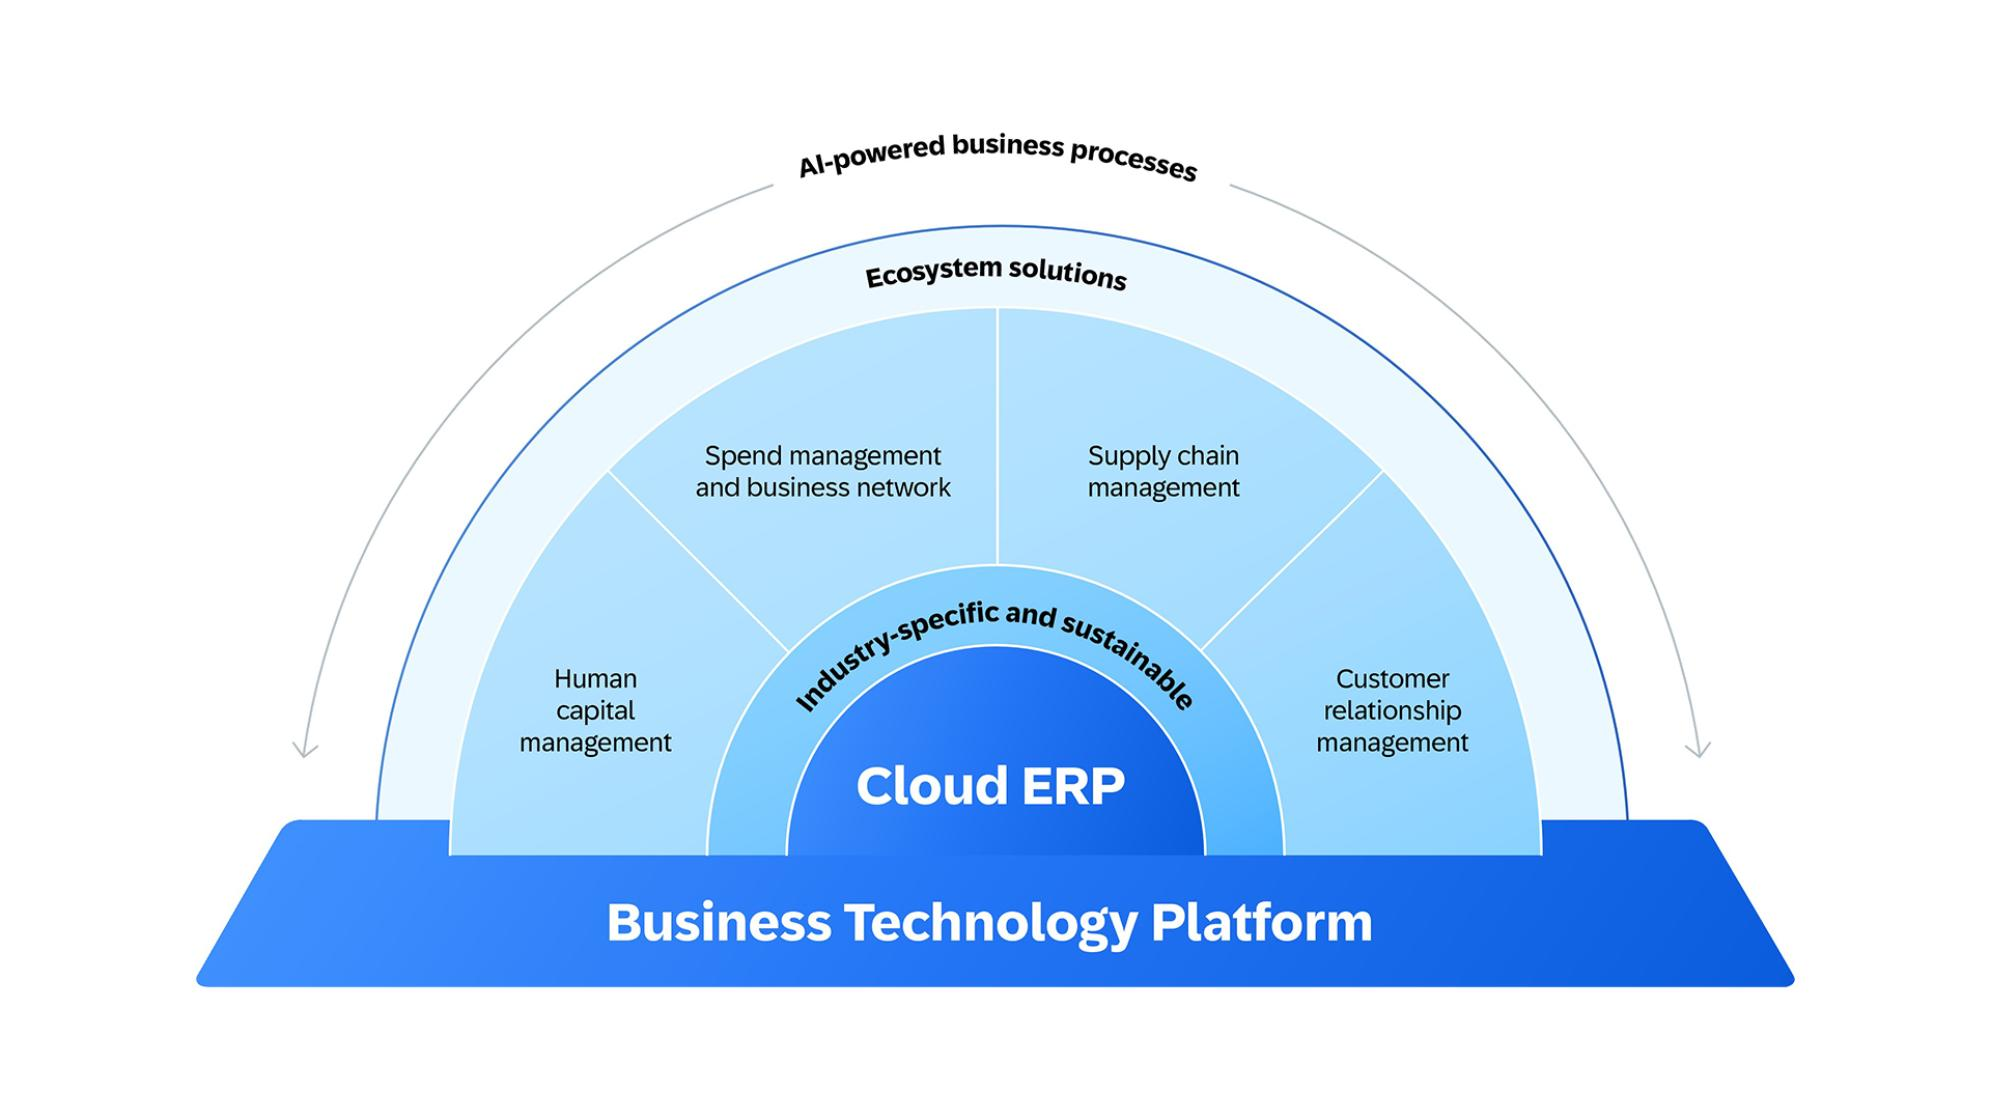
\includegraphics[scale=.21]{"bilder/produktportfolio.jpg"}
    \caption{Produktportfolio Übersicht von SAP}
    \footnotesize Quelle: \url{https://www.sap.com/intelligent-enterprise.html?url_id=banner-glo-homepage-row3-cta-who-we-are-230510}
    \label{fig:produktportfolio}
\end{figure}

Die SAP ist eine der größten Software-Entwicklungsunternehmen weltweit und hat, wie in Abbildung \Ref{fig:produktportfolio} dargestellt, ein sehr breites Produktportfolio für ein sehr breites Kundenfeld.
\cite{CorporateFactSheet}
Diese Produkte umfassen Bereich wie \gls{HR}, \gls{CRM}, Branchen spezifische Lösungen und noch vieles mehr.
Damit Kunden in der Benutzung eine klare und einheitliche Handhabung erfahren können, muss auch jedes Produkt als Software genauso gestaltet sein.
Nicht nur das -- sämtliche SAP Produkte sollten kongruent zueinander sein, da bei Kunden nicht das Gefühl entstehen darf, sie müssten mit jedem Produkt etwas komplett neuartiges erlernen.
Dies würde Kunden davon abhalten in weitere SAP Produkte zu investieren.
\cite{Hier ne passende quelle waere cool}

\end{document}